\chapter{Installing Quartus software.}
\graphicspath{ {./Lab00HowTo/howTo00 Install Quartus/Fig} }



To download and Install Quartus II and ModelSim on your home computer,
follow these instructions.

\begin{itemize}
\item
  Start
  at~\href{https://www.intel.com/content/www/us/en/software/programmable/quartus-prime/download.html}{this
  link}~to download Quartus.~
Link:
\url{https://www.intel.com/content/www/us/en/software/programmable/quartus-prime/download.html}
\item
  Click on the person icon in the upper right and either create an
  account or sign in with your existing account
\item
  Click on the "Download now" button for Lite Edition
\item
  Click the "18.1 (2)" link on the left side of the screen
\item
  Click the "Intel® Quartus® Prime Lite Edition Design Software Version
  18.1 for Windows"
\item
  On the redirect Download Center page click the "Download Quartus ...
  tar" button
\item
  Accept the license agreement
\item
  The approximately 5.8GB download should automatically start
\item
  Uncompress the zip file. If needed download and install WinZip to
  uncompress.
\item
  Double click on QuartusLiteSetup-18.1.0.625-windows and follow the
  prompts
\item
  Select the options given below


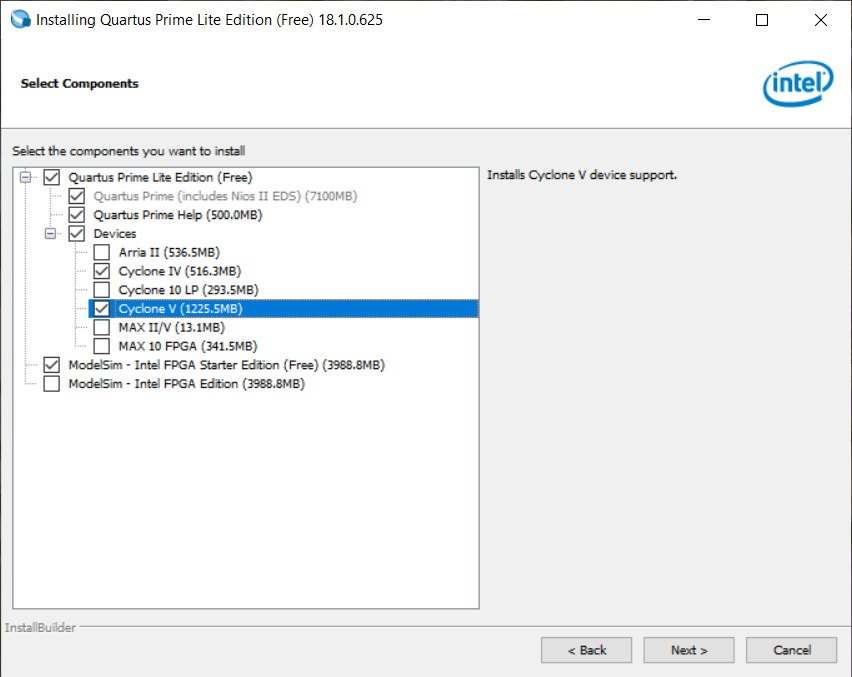
\includegraphics[width=0.4\paperwidth]{image1.png}

\item
  Install takes about 20 minutes.
\item
  Complete the install with the following options.


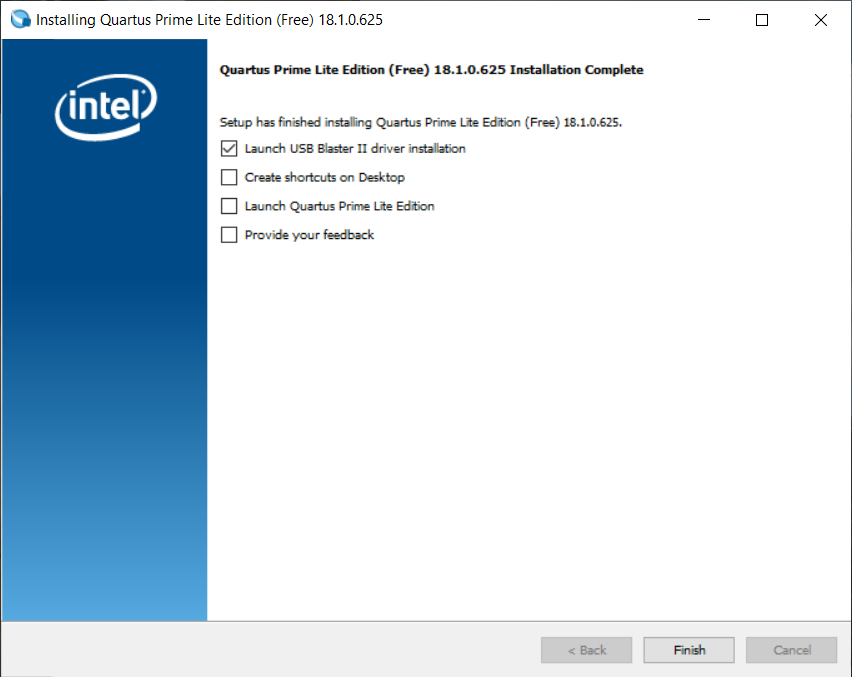
\includegraphics[width=0.4\paperwidth]{image2.png}


\item
  The Device Driver Wizard should auto launch after the install is
  finished, follow the prompt and finish.
\item
  You need to restart your computer to complete the installation.
\item
  When you run the Quartus software for the first time, you will be
  prompted to decide on a license. Select the option below.

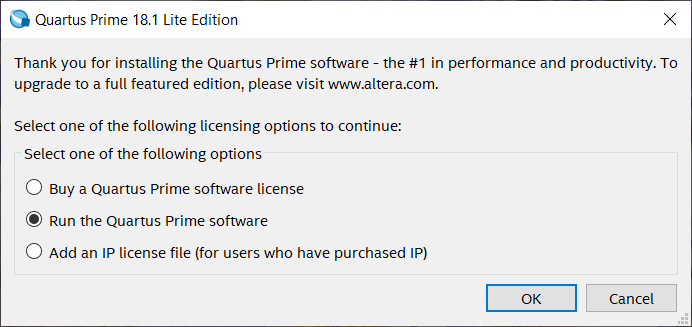
\includegraphics[width=0.4\paperwidth]{image3.png}

You should be ready to start using Quartus to write Verilog and use
ModelSim to check your designs.
\end{itemize}
